% ======================= CHAPTER 3: METHODOLOGY ==========================
\chapter{Methodology}

This chapter describes the experimental setup in detail, including the dataset characteristics, the selected model architectures, the optimization techniques employed, and the evaluation metrics used to assess model performance.

\section{Dataset: ISIC 2018 Challenge}

The dataset used in this study is the publicly available ISIC 2018 Skin Lesion Analysis Towards Melanoma Detection dataset (Task 3: Disease Classification). It contains 10,015 dermoscopy images distributed across seven diagnostic categories, as summarized in Table~\ref{tab:class_distribution}.

\begin{table}[H]
\centering
\caption{Class distribution of the ISIC 2018 dataset.}
\label{tab:class_distribution}
\begin{tabular}{llrrr}
\toprule
\textbf{Class} & \textbf{Full Name} & \textbf{Train} & \textbf{Val} & \textbf{Test} \\
\midrule
NV    & Melanocytic Nevus          & 4,693 & 1,006 & 1,006 \\
MEL   & Melanoma                   &   779 &   167 &   167 \\
BKL   & Benign Keratosis           &   769 &   165 &   165 \\
BCC   & Basal Cell Carcinoma       &   360 &    77 &    77 \\
AKIEC & Actinic Keratosis          &   229 &    49 &    49 \\
VASC  & Vascular Lesion            &    99 &    21 &    22 \\
DF    & Dermatofibroma             &    81 &    17 &    17 \\
\midrule
\textbf{Total} & & \textbf{7,010} & \textbf{1,502} & \textbf{1,503} \\
\bottomrule
\end{tabular}
\end{table}

The dataset exhibits a severe class imbalance, with NV constituting 66.9\% of the training samples while DF and VASC together represent only 2.6\%. This imbalance ratio of approximately 58:1 (NV to DF) poses a significant challenge for training unbiased classifiers. The data was split into training (70\%), validation (15\%), and test (15\%) sets with stratified sampling to preserve class proportions.

\begin{figure}[H]
\centering
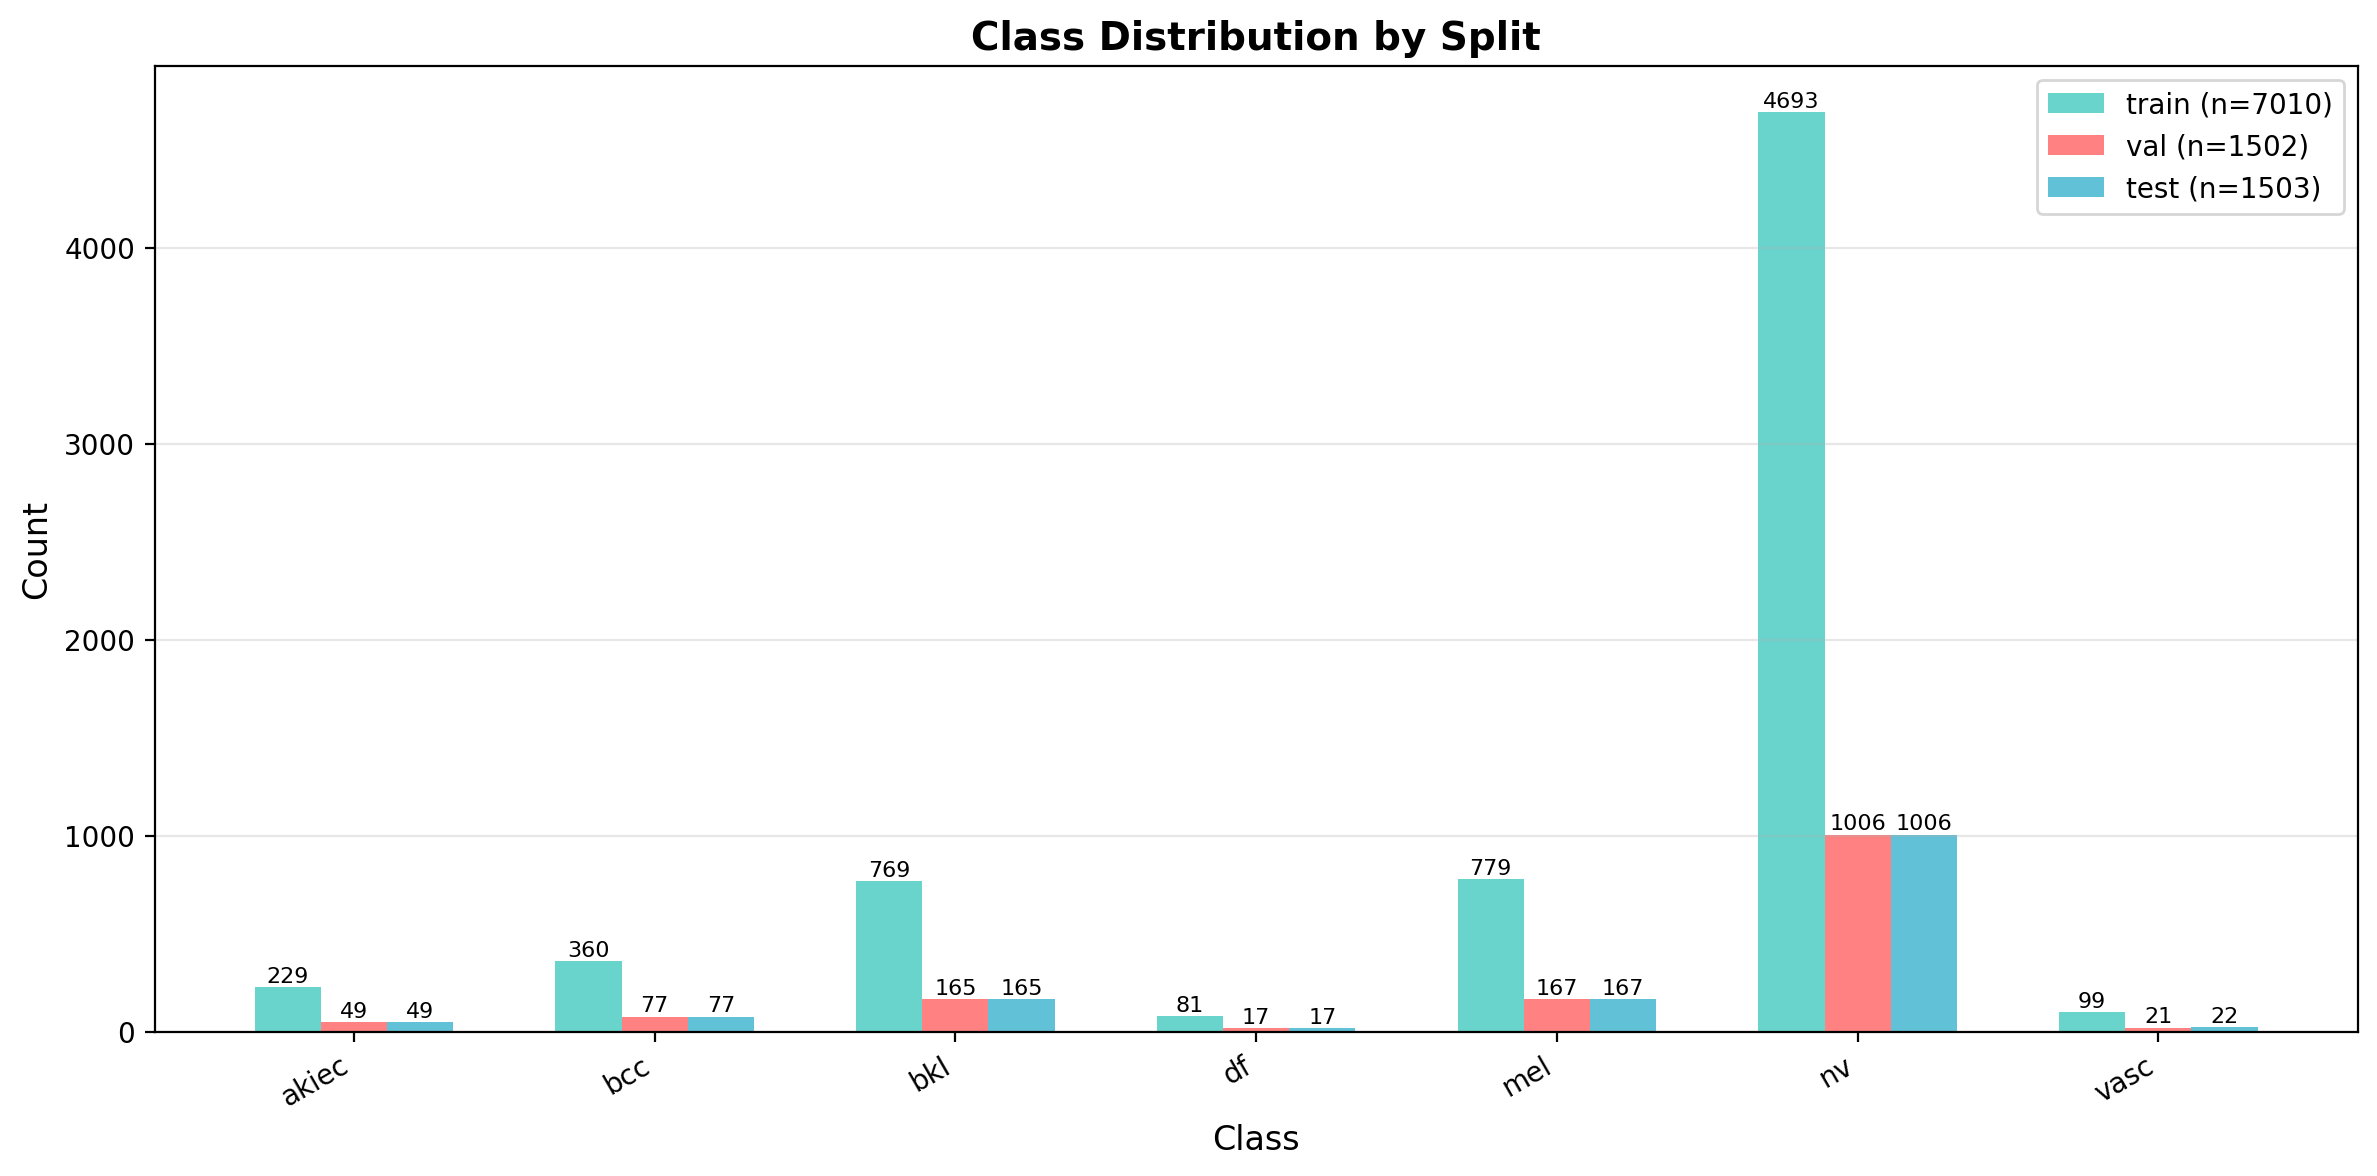
\includegraphics[width=\figwidth]{figures/class_distribution.png}
\caption{Class distribution across the training, validation, and test splits. The severe imbalance between NV and minority classes (DF, VASC) is clearly visible.}
\label{fig:class_distribution}
\end{figure}

\section{Model Architectures}

Four architectures were selected to represent a diverse spectrum of modern deep learning approaches: three CNNs and one Vision Transformer. All models were initialized with ImageNet-pretrained weights~\cite{deng2009imagenet} through the \texttt{timm} library~\cite{wightman2019timm} and fine-tuned on the ISIC 2018 dataset.

\subsection{EfficientNet-B0}

EfficientNet-B0 is the baseline model of the EfficientNet family, designed using Neural Architecture Search (NAS) and compound scaling~\cite{tan2019efficientnet}. With only 5.3 million parameters, it achieves competitive accuracy by jointly optimizing network depth, width, and resolution. In our pipeline, a dropout layer~\cite{srivastava2014dropout} ($p=0.3$) was added before the final classification head.

\subsection{ResNet50}

ResNet50 consists of 50 layers organized into four residual stages~\cite{he2016deep}. Its skip connections enable effective gradient flow during backpropagation, making it one of the most reliable architectures for transfer learning. With 25.6 million parameters, it is the second-largest model in our comparison. Dropout ($p=0.3$) was applied before the classifier.

\subsection{DenseNet121}

DenseNet121 features 121 layers with dense connectivity, where each layer receives concatenated feature maps from all preceding layers within the same dense block~\cite{huang2017densely}. This architecture promotes feature reuse and reduces parameter count to approximately 8 million. Due to the inherent regularization provided by dense connections, a slightly lower dropout ($p=0.25$) was used.

\subsection{Swin-Tiny}

Swin-Tiny is a hierarchical Vision Transformer that processes images through shifted window-based self-attention~\cite{liu2021swin}. Unlike CNNs, which rely on local receptive fields, Swin captures long-range dependencies through attention mechanisms. With 28 million parameters, it is the largest model evaluated. Following best practices for Transformer fine-tuning~\cite{touvron2021deit}, a lower learning rate ($1 \times 10^{-4}$) and higher weight decay (0.05) were used, along with an extended warmup period of 5 epochs.

\begin{table}[H]
\centering
\caption{Summary of the four evaluated architectures.}
\label{tab:architectures}
\begin{tabular}{lrllr}
\toprule
\textbf{Model} & \textbf{Params (M)} & \textbf{Type} & \textbf{Key Feature} & \textbf{Dropout} \\
\midrule
EfficientNet-B0 & 5.3  & CNN & Compound Scaling  & 0.30 \\
ResNet50        & 25.6 & CNN & Residual Connections & 0.30 \\
DenseNet121     & 8.0  & CNN & Dense Connectivity  & 0.25 \\
Swin-Tiny       & 28.0 & ViT & Shifted Window Attention & 0.30 \\
\bottomrule
\end{tabular}
\end{table}

\section{Training Pipeline}

An optimized training pipeline was developed to maximize model generalization and address the challenges of class imbalance. The pipeline integrates multiple complementary techniques, each targeting a specific aspect of the training process.

\subsection{Weighted Random Sampling}

To counteract class imbalance during training, a Weighted Random Sampler was employed. Each sample is assigned a weight inversely proportional to the frequency of its class in the training set:

\begin{equation}
w_c = \frac{N}{C \cdot n_c}
\label{eq:class_weight}
\end{equation}

where $N$ is the total number of training samples, $C$ is the number of classes, and $n_c$ is the number of samples belonging to class $c$. This ensures that mini-batches are approximately class-balanced, preventing the model from developing a bias toward the majority class (NV).

\subsection{Mixup and CutMix Augmentation}

To further regularize training and improve generalization, Mixup and CutMix were applied with equal probability ($p=0.5$ each) during training.

\textbf{Mixup} creates virtual training examples by linearly interpolating pairs of images and their labels:
\begin{equation}
\tilde{x} = \lambda x_i + (1 - \lambda) x_j, \quad \tilde{y} = \lambda y_i + (1 - \lambda) y_j
\label{eq:mixup}
\end{equation}
where $\lambda \sim \text{Beta}(\alpha, \alpha)$ with $\alpha = 0.2$.

\textbf{CutMix} replaces a rectangular patch of one image with the corresponding patch from another, adjusting the label proportionally to the area of the patch:
\begin{equation}
\tilde{x} = M \odot x_i + (1 - M) \odot x_j, \quad \tilde{y} = \lambda y_i + (1 - \lambda) y_j
\label{eq:cutmix}
\end{equation}
where $M$ is a binary mask indicating the cut region and $\lambda$ equals the ratio of the unmasked area. The CutMix alpha was set to 1.0.

These augmentations force the model to learn from mixed signals, discouraging memorization and encouraging smoother decision boundaries.

\subsection{Label Smoothing}

Standard one-hot encoded labels assign a probability of 1.0 to the correct class and 0.0 to all others. Label Smoothing redistributes a small fraction of the probability mass to incorrect classes:
\begin{equation}
y_{\text{smooth}} = (1 - \epsilon) \cdot y_{\text{one-hot}} + \frac{\epsilon}{C}
\label{eq:label_smooth}
\end{equation}
where $\epsilon = 0.1$ is the smoothing factor and $C = 7$ is the number of classes. This technique prevents the model from becoming overconfident in its predictions, which improves calibration and AUC scores.

\subsection{Optimization and Scheduling}

All models were trained using the AdamW optimizer~\cite{loshchilov2019decoupled}, which decouples weight decay from the gradient update, leading to better generalization compared to standard Adam. A cosine annealing schedule with linear warmup~\cite{loshchilov2017sgdr} was employed:

\begin{itemize}
    \item \textbf{Warmup phase} (first 3--5 epochs): The learning rate increases linearly from a near-zero value to the target learning rate, preventing early instability when the randomly initialized classification head produces large gradients.
    \item \textbf{Cosine decay phase} (remaining epochs): The learning rate decreases following a cosine curve to a minimum value of $1 \times 10^{-6}$, allowing the model to settle into a flat minimum of the loss landscape.
\end{itemize}

\subsection{Data Augmentation}

Beyond Mixup and CutMix, the following standard augmentations were applied during training:
\begin{itemize}
    \item Random horizontal and vertical flips ($p=0.5$)
    \item Random rotation (up to $\pm90^\circ$)
    \item Color jittering (brightness, contrast, saturation, hue; magnitude 0.25)
    \item Random Resized Crop (scale range: 0.85--1.0)
    \item Gaussian Blur ($p=0.1$)
    \item Random Erasing ($p=0.1$)
\end{itemize}

All images were resized to $224 \times 224$ pixels and normalized using ImageNet mean and standard deviation values~\cite{deng2009imagenet}. A batch size of 16 was selected to accommodate GPU memory constraints when running all four architectures (including the 28M-parameter Swin-Tiny) under identical conditions with mixed-precision training, ensuring a fair and consistent comparison across all experiments.

\begin{table}[H]
\centering
\caption{Hyperparameter configuration for each model.}
\label{tab:hyperparams}
\begin{tabular}{lcccc}
\toprule
\textbf{Hyperparameter} & \textbf{EB0} & \textbf{RN50} & \textbf{DN121} & \textbf{Swin-T} \\
\midrule
Learning Rate        & 3e-4  & 3e-4  & 2.5e-4 & 1e-4 \\
Weight Decay         & 1e-3  & 1e-3  & 1e-3   & 5e-2 \\
Warmup Epochs        & 3     & 3     & 3      & 5 \\
Max Epochs           & 50    & 50    & 50     & 50 \\
Batch Size           & 16    & 16    & 16     & 16 \\
Early Stopping       & 12    & 12    & 12     & 12 \\
Mixup $\alpha$       & 0.2   & 0.2   & 0.2    & 0.2 \\
CutMix $\alpha$      & 1.0   & 1.0   & 1.0    & 1.0 \\
Label Smoothing      & 0.1   & 0.1   & 0.1    & 0.1 \\
\bottomrule
\end{tabular}
\end{table}

\section{Evaluation Metrics}

Given the severe class imbalance, accuracy alone is an insufficient measure of model performance. A model that simply predicts NV for every input would achieve approximately 67\% accuracy. Therefore, we report a comprehensive set of metrics:

\begin{itemize}
    \item \textbf{Macro F1-Score:} The unweighted mean of per-class F1-scores, giving equal importance to all classes regardless of their frequency. This is our primary selection metric.
    \item \textbf{Area Under the ROC Curve (AUC):} Measures the model's ability to discriminate between classes across all possible decision thresholds. A macro-averaged AUC close to 1.0 indicates excellent probability calibration.
    \item \textbf{Cohen's Kappa ($\kappa$):} Measures agreement between predicted and true labels, correcting for chance agreement. Values above 0.6 indicate substantial agreement.
    \item \textbf{Matthews Correlation Coefficient (MCC):} A balanced measure that accounts for all four entries of the confusion matrix (TP, TN, FP, FN), considered the most informative single metric for imbalanced classification.
    \item \textbf{Per-class Sensitivity and Specificity:} Sensitivity (recall) measures the proportion of actual positives correctly identified, while specificity measures the proportion of actual negatives correctly identified. Both are critical in medical diagnostics.
\end{itemize}

\section{Ensemble Strategy}

After training all four models independently, we constructed an ensemble using soft voting. For each test sample, the softmax probability vectors from all four models were averaged element-wise, and the final prediction was taken as the class with the highest averaged probability:

\begin{equation}
\hat{y} = \arg\max_c \frac{1}{M} \sum_{m=1}^{M} p_m(c \mid x)
\label{eq:ensemble}
\end{equation}

where $M=4$ is the number of models and $p_m(c \mid x)$ is the probability assigned to class $c$ by model $m$. This approach leverages the complementary strengths of different architectures: CNNs provide strong local feature extraction while the Transformer captures global spatial relationships.

\section{Model Interpretability with Grad-CAM}

To ensure that the trained models attend to clinically meaningful regions, Gradient-weighted Class Activation Mapping (Grad-CAM)~\cite{selvaraju2017grad} was applied. Given a target class $c$, Grad-CAM computes the gradient of the class score $y^c$ with respect to the feature maps $A^k$ of the last convolutional layer:

\begin{equation}
\alpha_k^c = \frac{1}{Z} \sum_i \sum_j \frac{\partial y^c}{\partial A_{ij}^k}
\label{eq:gradcam_weights}
\end{equation}

The final heatmap is obtained by computing a weighted combination of the feature maps followed by a ReLU activation:

\begin{equation}
L_{\text{Grad-CAM}}^c = \text{ReLU}\left(\sum_k \alpha_k^c A^k\right)
\label{eq:gradcam}
\end{equation}

This produces a coarse localization map highlighting regions that positively influence the prediction for class $c$. The heatmap is then upsampled to the input image resolution and overlaid as a color-coded visualization.
